\documentclass[a4paper]{article}
\usepackage[utf8x]{inputenc}
\usepackage[portuguese]{babel}
\usepackage{graphicx}
\usepackage{a4wide}
\usepackage[pdftex,hidelinks]{hyperref}
\usepackage{float}
\usepackage{indentfirst}
\usepackage{subcaption}
\usepackage[cache=false]{minted}
\usepackage{amsmath}
\usepackage{listings}
\usepackage{color}
\usepackage{gensymb}
\usepackage{tikz}

\definecolor{dkgreen}{rgb}{0,0.6,0}
\definecolor{gray}{rgb}{0.5,0.5,0.5}
\definecolor{mauve}{rgb}{0.58,0,0.82}

\lstset{frame=tb,
language=C++,
aboveskip=3mm,
belowskip=3mm,
showstringspaces=false,
columns=flexible,
basicstyle={\small\ttfamily},
numbers=none,
numberstyle=\tiny\color{gray},
keywordstyle=\color{blue},
commentstyle=\color{dkgreen},
stringstyle=\color{mauve},
breaklines=true,
breakatwhitespace=true,
tabsize=4
}

\newcommand{\x}{\times}

\begin{document}

\title{Computação Gráfica\\ Animações}
\author{Bárbara Cardoso (a80453) \and Márcio Sousa (a82400)
\and Pedro Mendes (a79003)}
\date{\today}

\begin{titlepage}

    %título
    \thispagestyle{empty}
    \begin{center}
        \begin{minipage}{0.75\linewidth}
            \centering
            %engenharia logo
            
\includegraphics[width=0.4\textwidth]{eng.jpeg}\par\vspace{1cm}
            \vspace{1.5cm}
            %títulos
            \href{https://www.uminho.pt/PT}
            {\scshape\LARGE Universidade do Minho} \par
            \vspace{1cm}
            \href{https://www.di.uminho.pt/}
            {\scshape\Large Departamento de Informática} \par
            \vspace{1.5cm}

            \maketitle
        \end{minipage}
    \end{center}

\end{titlepage}

\tableofcontents

\pagebreak

\section{Introdução}
Este trabalho foi proposto no âmbito da unidade curricular de Computação
Gráfica, e tem como objetivo desenvolver um motor gráfico genérico para
representar objetos a 3 dimensões. Este relatório tem como contexto ambos os
relatórios anteriores.

Nesta quarta fase do projeto estendemos as capacidades do motor gráfico
anteriormente definido com a adição de luzes e texturas. Foram também feitas
algumas otimizações a este.

O gerador de modelos foi também estendido para calcular para cada uma das
primitivas os vetores normais e as coordenadas de textura das mesmas.

Por fim, o modelo de teste utilizado (O Sistema Solar) foi alterado para
demonstrar estas capacidades, fazendo uso de texturas para os planetas e Sol,
assim como colocar iluminação neste.


\section{Generator}

O output do \textit{generator} foi alterado para incluir as normais e as
coordenadas de textura correspondentes aos pontos dos triângulos calculados.
Em seguida, passamos a explicar o processo do cálculo das normais e das
coordenadas de textura para cada uma das primitivas.

\subsection{Nova Primitiva: Cilindro}

Foi adicionado ao gerador a primitiva cilindro. Este é definido pelo raio da
base, altura e número de \textit{slices}.

Em cada iteração são definidos quatro pontos usando coordenadas polares, estes
quatro pontos são os cantos da slice respectiva, depois usando estes são
desenhados quatro triângulos, um para a base, outro para o topo e por fim
outros dois para a fazer o rectângulo que compõem a \textit{slice}.

\begin{figure}[H]
    \centering
    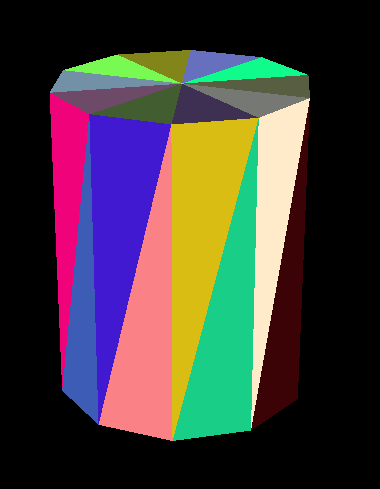
\includegraphics[width=0.3\textwidth]{cylinder_colored.png}
    \caption{Cilindro gerado com 10 slices}
\end{figure}

\subsection{Vetores Normais e Coordenadas de Textura}

\subsubsection{Plano}
Como um plano está situado no plano xOz e as normais são sempre vetores
perpendiculares, as normais deste são vetores unitários com apenas a componente
y positiva.

As coordenadas de textura para o plano são calculadas de forma
muito simples. Como o plano e a textura tem a mesma forma, o mapeamento é
directo, assim, os cantos da textura são mapeados para os cantos do plano.

\begin{figure}[H]
    \centering
    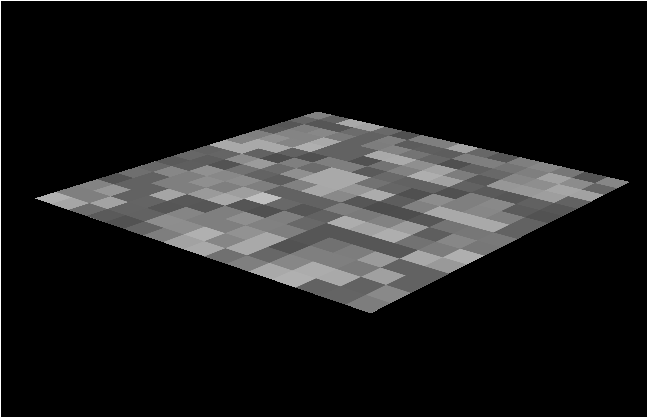
\includegraphics[width=0.7\textwidth]{plane.png}
    \caption{Plano com textura}
\end{figure}

\subsubsection{Cubo}
As normais de um cubo também são simples de calcular, pois cada uma das faces é
paralela a um dos planos (xOz, xOy, yOz), logo as normais dessa face são
perpendiculares ao plano correspondente.

Para as texturas começou-se por definir uma fórmula que mapeasse as coordenadas
de cada face para valores compreendidos entre, 0 e $\frac{1}{3}$ e 0 e
$\frac{1}{2}$, dependendo do eixo pretendido. Depois é somado um
\textit{offset} a estes valores dependendo da secção da textura que se pretende
mapear.

Assumindo que o ponto de vista é colocado em (0,0,1), as coordenadas de textura
da face da frente são $x \in [0,\frac{1}{3}]$ e $y \in [0,\frac{1}{2}]$ logo o
\textit{offset} destes é nulo. No entanto, para a face da esquerda, as suas
coordenadas de textura são $x \in [\frac{2}{3},1]$ e $y \in [\frac{1}{2},1]$,
logo o \textit{offset} destes é $\frac{2}{3}$ e $\frac{1}{2}$, respetivamente.

\begin{figure}[H]
    \centering
    \usetikzlibrary{matrix,backgrounds,positioning,calc,fit}
\definecolor{SceneColor}{RGB}{200,200,200}
\definecolor{GroupColor}{RGB}{90,200,102}
\definecolor{SubGroupColor}{RGB}{114,247,247}

\begin{tikzpicture}[font=\ttfamily,
    array/.style={matrix of nodes,
    nodes={draw=none, minimum width=16mm, minimum height=5mm, fill=white},
    column sep=-\pgflinewidth,
    row sep=-\pgflinewidth,
    nodes in empty cells,
    row 1/.style={nodes={draw=none, fill=none, minimum size=5mm}}}]

    \matrix[array] (Cube) {
        (0,0) &  & (0.333, 0) &  & (0.666,0.0) &  & (1,0) \\
        & F $\downarrow$ &           &  U $\downarrow$ &            & R $\to$ &      \\
        (0,0.5) &  & (0.333, 0.5) &  & (0.666,0.5) &  & (1,0.5) \\
        & B $\downarrow$ &           &  D $\downarrow$ &            & L $\to$ &      \\
        (0,1) &  & (0.333, 1) &  & (0.666,1.0) &  & (1,1) \\
    };

    \foreach \from/\to in {
        Cube-1-1/Cube-1-3, Cube-1-3/Cube-1-5, Cube-1-5/Cube-1-7,
        Cube-3-1/Cube-3-3, Cube-3-3/Cube-3-5, Cube-3-5/Cube-3-7,
        Cube-5-1/Cube-5-3, Cube-5-3/Cube-5-5, Cube-5-5/Cube-5-7,
        Cube-1-1/Cube-3-1, Cube-1-3/Cube-3-3, Cube-1-5/Cube-3-5, Cube-1-7/Cube-3-7,
        Cube-3-1/Cube-5-1, Cube-3-3/Cube-5-3, Cube-3-5/Cube-5-5, Cube-3-7/Cube-5-7}
    \draw [<->, thick] (\from)--(\to);

    % \matrix[array, below = of Scene] (Group2) {
    %     Group 2 \\
    %     Model 4 & Model 5 \\
    %     \\
    % };

    % \matrix[array, left = of Group2] (Group1) {
    %     &  Group 1 & \\
    %     Model 1 & Model 2 & Model 3 \\
    % };

    % \matrix[array, right = of Group2] (Group3) {
    %     Group 3 \\
    %     Model 7 \\
    % };

    % \matrix[array, below = of Group2] (Group21) {
    %     Group 2.1 \\
    %     Model 6 \\
    % };

    % \node[draw, fill=GroupColor, minimum size=2mm, circle] at (Scene-2-1) (Group1Ball) {};
    % \node[draw, fill=GroupColor, minimum size=2mm, circle] at (Scene-2-2) (Group2Ball) {};
    % \node[draw, fill=GroupColor, minimum size=2mm, circle] at (Scene-2-3) (Group3Ball) {};
    % \node[draw, fill=SubGroupColor, minimum size=2mm, circle] at (Group2-3-1) (Group21Ball) {};

    % \begin{scope}[on background layer]
    %     \node[draw, fill=SceneColor, fit = (Scene) (Group1) (Group2) (Group3) (Group21)]
    %     (SceneBox) {};
    %     \node[draw, fill=GroupColor, fit = (Group1)] (Group1Box) {};
    %     \node[draw, fill=GroupColor, fit = (Group2) (Group21)] (Group2Box) {};
    %     \node[draw, fill=GroupColor, fit = (Group3)] (Group3Box) {};
    %     \node[draw, fill=SubGroupColor, fit = (Group21)] (Group21Box) {};
    % \end{scope}

    % \foreach \from/\to in {
    %     Group1Ball/Group1Box, Group2Ball/Group2Box,
    %     Group3Ball/Group3Box, Group21Ball/Group21Box}
    % \draw [->, thick] (\from)--(\to);

\end{tikzpicture}

    \caption{Esquema de como a textura deve ser desenhada.}
\end{figure}

\begin{figure}[H]
    \centering
    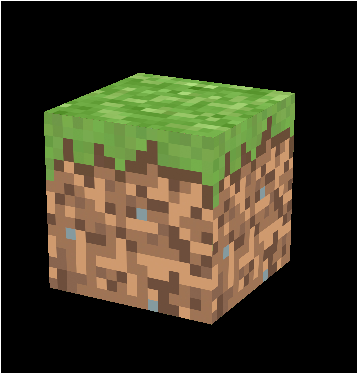
\includegraphics[width=0.5\textwidth]{box.png}
    \caption{Plano com textura}
\end{figure}

\subsubsection{Esfera}\label{sec:esfera}
Sendo que a esfera está sempre centrada na origem, para calcular as normais
desta, é preciso apenas normalizar as coordenadas dos pontos de forma a obter
as normais.

A textura usada para aplicar à esfera é rectangular, assim, o raciocínio
utilizado para aplicar a textura é imaginar que a esfera é cortada em altura e
``espalmada'' sobre a textura, de seguida é apenas necessário mapear
directamente a textura sobre estar interpretação da esfera.

\begin{figure}[H]
    \centering
    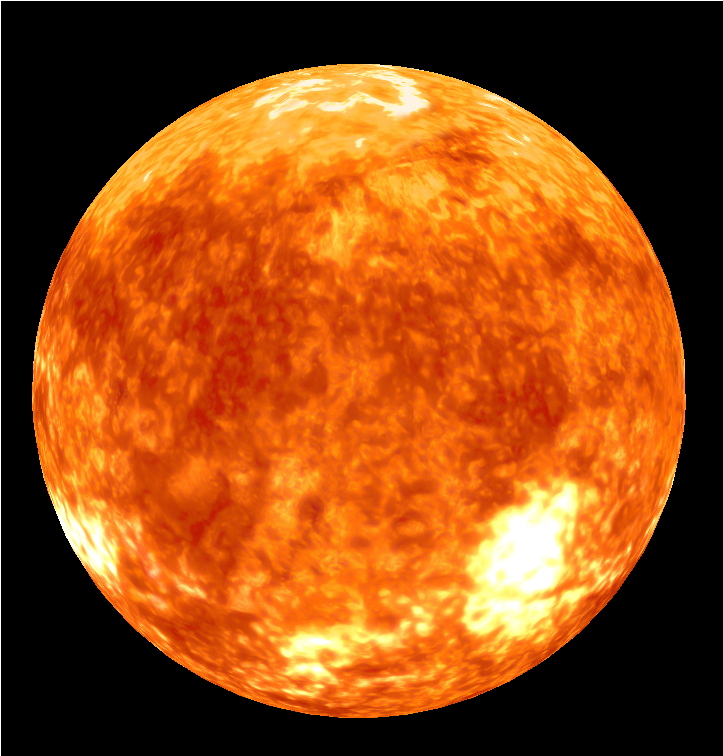
\includegraphics[width=0.7\textwidth]{sphere.png}
    \caption{Plano com textura}
\end{figure}

\subsubsection{Cone}
O cálculo das normais do cone é feito em duas partes, primeiro são calculadas
as normais da base, que por definição são o vector unitário $(0,-1,0)$. A
segunda parte corresponde ao lado do cone, para o qual é calculado o ângulo
entre qualquer ponto do lado do cone e a base do mesmo através da
$\arctan(\frac{radius}{stacks})$, este ângulo define a
inclinação das normais laterais. Depois disto, basta utilizar coordenadas
polares para determinar as componentes $x$ e $z$ do vetor e normalizar.

Para aplicar uma textura a um cone foi definido o formato da
figura~\ref{fig:conetexture}, ou seja, a metade esquerda da imagem é a base do
cone, e a metade direita é a textura do lado do cone. Depois a textura é
dividida no mesmo número de \textit{slices} e \textit{stacks} que o cone tem e
faz-se o mapeamento.

\begin{figure}[H]
    \centering
    \includegraphics{../assets/cone_rain.png}
    \caption{Textura exemplo de um cone}\label{fig:conetexture}
\end{figure}

\begin{figure}[H]
    \centering
    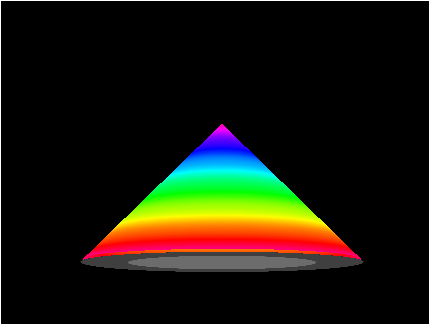
\includegraphics[width=0.7\textwidth]{cone.png}
    \caption{Plano com textura}
\end{figure}

\subsection{Cilindro}
As normais dos cilindro são relativamente simples, para a base e topo as
normais são sempre $(0,-1,0)$ e $(0,1,0)$ respetivamente, para o lado, é apenas
necessário normalizar as coordenadas dos pontos respetivos depois de colocar o
seu $y$ a 0 (para que seja paralelo ao plano xOz).

Para as coordenadas de textura é foi utilizado o \textit{template} da
figura~\ref{fig:cilindro}. Para os lados divide-se o rectângulo pelo número de
\textit{slices} e sempre que se avança de \textit{slice} soma-se essa quantidade
ao $x$ da textura. O $y$ so toma dois valores 0 e 0.625. Por fim, o topo e a
base são obtidas através de coordenadas polares, somando ao centro de cada uma
$\sin(\alpha) \times 0.1875$ para o $x$ e $\cos(alpha) \times 0.1875$ para o $y$.

\begin{figure}[H]
    \centering
    \includegraphics{../assets/OilBarrel.jpg}
    \caption{Exemplo de um template possível para o
    cilindro.}\label{fig:cilindro}
\end{figure}

\begin{figure}[H]
    \centering
    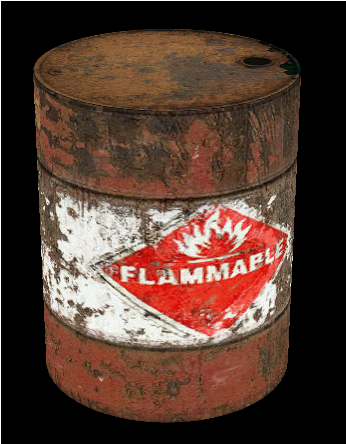
\includegraphics[width=0.5\textwidth]{cylinder.png}
    \caption{Plano com textura}
\end{figure}

\subsubsection{Torus}
As normais do torus fazem uso da mesma técnica utilizada para a esfera,
(Ver~\ref{sec:esfera}) apenas alterado o centro, agora a origem já não é o
ponto de referência mas sim os centros de cada anel do torus, visto que o
raciocínio para o cálculo dos pontos deste já era vetorial, foi apenas
necessário normalizar os vetores.

Para as coordenadas de textura, o mapeamento é também similar ao da esfera,
imagina-se que a \textit{mesh} do torus é espalmada sobre a textura deste, e
assim o mapeamento é direto. Percorrer a textura ao longo do eixo dos $y$
implica percorrer o torus à volta do seu perímetro enquanto que no eixo dos $x$
desenha-se cada anel do torus.

\begin{figure}[H]
    \centering
    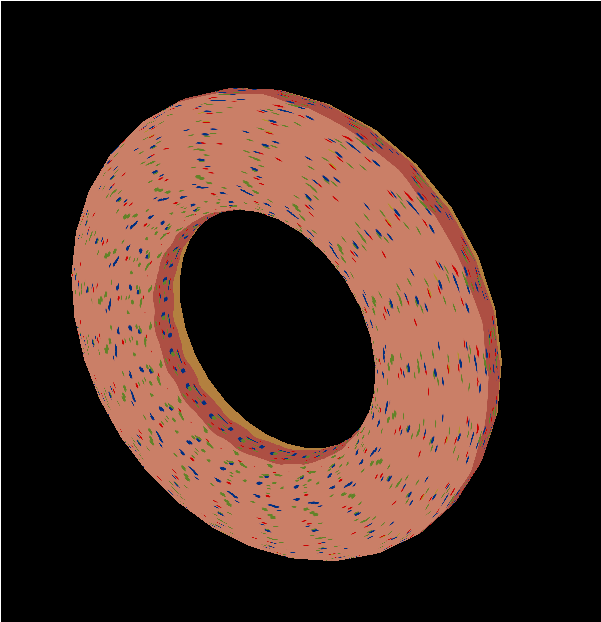
\includegraphics[width=0.5\textwidth]{torus.png}
    \caption{Plano com textura}
\end{figure}

\subsubsection{\textit{Bezier Patches}}

Para calcular as normais do \textit{Bezier patch} usa se o mesmo algoritmo de
calculo usado para os pontos, mas em vez de calcular um ponto calcula-se dois
vetores tangentes a este e com o produto escalar encontra-se o vetor normal ao
ponto.

\begin{figure}[H]
    \centering
    \includegraphics[width=0.5\textwidth]{bez-normal.png}
    \caption{Calculo da normal através dos vetores tangentes.}
\end{figure}

Para as coordenadas de textura, simplesmente mapea-se a textura toda para cada
superfície de \textit{Bezier}. Ficando assim repetida tantas vezes quantos os
patches do modelo.

\begin{figure}[H]
    \centering
    \begin{subfigure}{0.4\textwidth}
        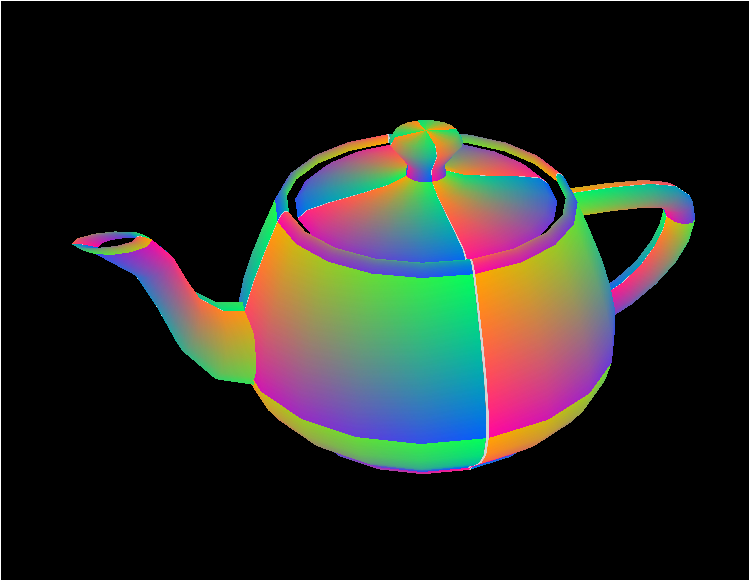
\includegraphics[width=\textwidth]{./teapot.png}
        \caption{Teapot}
    \end{subfigure}
    \begin{subfigure}{0.4\textwidth}
        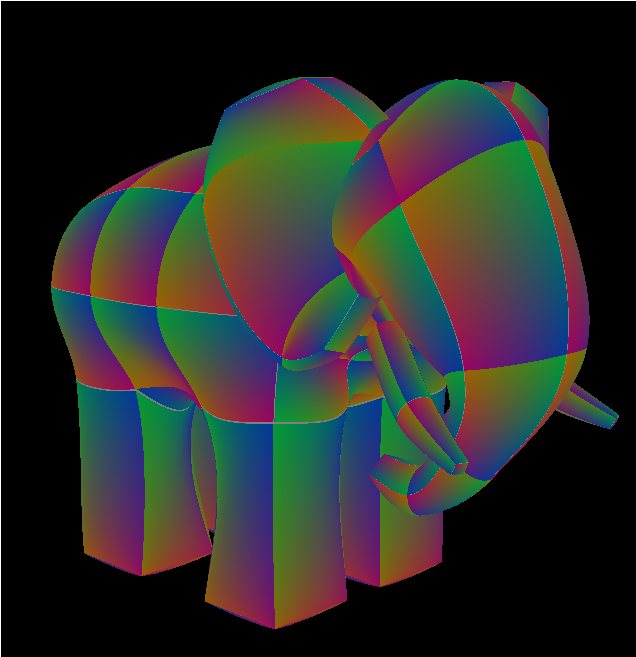
\includegraphics[width=\textwidth]{./gumbo.png}
        \caption{Gumbo}
    \end{subfigure}
    \caption{Exemplos de modelos gerados por patches}
\end{figure}

\section{Engine}

O \textit{engine} foi estendido para possibilitar a renderização de
modelos com superfícies mais complexas, permitindo definir se um objeto tem uma
superfície difusa, especular, emissiva e/ou ambiente, assim como definir uma
textura para a cobrir.

\subsection{Sem texturas}
A entrada de um \textit{model} no XML pode agora incluir as componentes acima
referidas através das propriedades \texttt{ambi[RGB]}, \texttt{diff[RGB]},
\texttt{spec[RGB]} e \texttt{emis[RGB]}. Por exemplo,\\
\verb!<model file="models/sphere.3d" ambiR="0.2" diffB="0.8" />!

Todas as componentes têm valores por defeito de $(0,0,0)$ exceto a componente
difusa que tem $(1,1,1)$ por defeito. Num esforço de manter \textit{backwards
compatibility} e cenas de fases anteriores continuarem a funcionar, quando
nenhuma componente é especificada a cor do grupo é passada como valor da
componente emissiva dos seus \textit{models}.

\subsection{Com texturas}

Para além das componentes, pode ser passado também o ficheiro de onde carregar
a textura do modelo utilizando o atributo \texttt{texture}. Por exemplo\\
\verb!<model file="models/sphere.3d" texture="assets/8k_jupiter.jpg" />!

\section{Lighting}

Este programa oferece 3 tipos de luzes, pontual, direccional e
\textit{spotlight}. Estas são afectadas  por transformações geométricas como
qualquer outro objecto e podem ser definidas tanto ao nível de cena
(\texttt{<scene>}) como ao nível de um qualquer grupo, tendo em atenção que
apenas 8 luzes podem ser carregadas pelo programa.

Cada uma com os seus parâmetros específicos que serão delineados nas subsecções
seguintes.

\subsection{\textit{Point Light}}

Para definir uma luz pontual tem de ser passado o atributo \texttt{type} com o
valor \texttt{POINT}. Os parâmetros admitidos pela luz pontual são:

\begin{itemize}
    \item \textbf{Posicao}: Através dos atributos \texttt{posX}, \texttt{posY},
        e \texttt{posZ}.
    \item \textbf{Cor}: Através dos atributos \texttt{R}, \texttt{G} e
        \texttt{B}.
\end{itemize}

\subsection{\textit{Directional Light}}

Para definir uma luz direccional tem de ser passado o atributo \texttt{type}
com o valor \texttt{DIRECTIONAL}. Os parâmetros admitidos pela luz pontual são:

\begin{itemize}
    \item \textbf{Direcção}: Através dos atributos \texttt{dirX}, \texttt{dirY}
        e \texttt{dirZ}.
    \item \textbf{Cor}: Através dos atributos \texttt{R}, \texttt{G} e
        \texttt{B}.
\end{itemize}

\subsection{\textit{Spotlight}}

Para definir uma luz \textit{spotlight} tem de ser passado o atributo
\texttt{type} com o valor \texttt{SPOT}. Os parâmetros admitidos pela luz
pontual são:

\begin{itemize}
    \item \textbf{Posição}: Através dos atributos \texttt{posX}, \texttt{posY},
        e \texttt{posZ}.
    \item \textbf{Direcção}: Através dos atributos \texttt{dirX}, \texttt{dirY}
        e \texttt{dirZ}.
    \item \textbf{Cor}: Através dos atributos \texttt{R}, \texttt{G} e
        \texttt{B}.
\end{itemize}

\section{Sistema Solar}
O sistema solar foi alterado para aplicar uma textura a cada astro e uma luz
pontual no centro do Sol.

\section{Optimizações}
Para otimizar a utilização de memória do programa, foi criada uma cache de
modelos e texturas, assim cada conjunto de pontos, normais e coordenadas de
textura, correspondente a um ficheiro \texttt{.3d}, é carregado apenas uma vez
para o GPU e reutilizado para todos os modelos que os utilizam. O mesmo
raciocínio foi feito para as texturas, para que não fosse lido para memória
mais do que uma cópia de cada textura.

Para o caso do sistema solar, como todos os planetas utilizam o mesmo modelo
unitário da esfera, independentemente de quantos astros sejam colocados no
modelo, o ficheiro \texttt{sphere.3d} é lido apenas uma vez.

\section{Conclusões e Trabalho Futuro}

Em conclusão, a área de computação gráfica apresenta desafios bastante
diferentes das outras áreas de ciências de computação, tanto no que toca a
gestão de memória e de recursos de computação, como também nos conhecimentos de
geometria e álgebra.

Como trabalho futuro, poderiam ser feitas várias otimizações como oclusão e a
utilização de índices para melhorar o desempenho dos VBOs.

\end{document}
